\documentclass[usenames,dvipsnames]{beamer}
\usepackage{../../shared/styles/custom}
\usepackage{../../shared/styles/conventions}
\usepackage{../../shared/notation/notation}

\title{Conventions, Accuracy Metrics, Classification, Regression}
\date{\today}
\author{Nipun Batra and teaching staff}
\institute{IIT Gandhinagar}
\begin{document}
  \setcounter{popquiz}{0}

  \maketitle
  
  % Table of Contents
  \begin{frame}{Outline}
    \tableofcontents
  \end{frame}
  
    \section{Introduction and Demos}
  
  \begin{frame}{Demo}
	Comet browser and automation of tasks
  \end{frame}
  

 
  \begin{frame}{Revision: What is Machine Learning}
	 ``Field of study that gives computers the ability to learn
		without being explicitly programmed'' - Arthur Samuel
		[1959]

		\pause Let us work on the digit recognition problem.

		\begin{figure}[htp]
			\centering
			\begin{notebookbox}{https://nipunbatra.github.io/ml-teaching/notebooks/rule-based-vs-ml.html}
			  \includegraphics[scale=0.35]{../assets/accuracy-convention/figures/mnist.pdf}
			\end{notebookbox}
		  \end{figure}
	\end{frame}
		
	

\begin{frame}{Revision: What is Machine Learning}
\cleanitemize{
	\item How would you program to recognise digits? Start with 4.
	\item Maybe 4 can be thought of as: $\bm{|}$ + $\bm{\rule[0.5ex]{1em}{.95pt}}$ + $\bm{|}$ + another vertically down $\bm{|}$
	\item The heights of each of the $\bm{|}$ need to be similar within tolerance
	
	\item Each of the $\bm{|}$ can be slightly slanted. Similarly the horizontal line can be slanted.
	\item There can be some cases of 4 where the first $\bm{|}$ is at 45 degrees
	\item There can be some cases of 4 where the width of each stroke is different
}
\end{frame}	
  
 
\section{Machine Learning Fundamentals}

\begin{frame}{Traditional Programming vs Machine Learning}
\begin{center}
\begin{tikzpicture}[node distance=2cm]
  \node (D1) [startstop] {Data};
  \node (R1) [startstop, below of=D1] {Rules};
  \node (T1) [startstop, right of=D1, xshift=2cm, yshift=-1cm] {\makecell[l]{Traditional\\Programming}};
  \node (A1) [startstop, right of=T1, xshift=2cm] {Answers};
  \draw [arrow] (D1) -- (T1);
  \draw [arrow] (R1) -- (T1);
  \draw [arrow] (T1) -- (A1);
\end{tikzpicture}
\end{center}
\end{frame}


\begin{frame}{Traditional Programming}
\begin{tikzpicture}[node distance=2cm]
  \node (Data1) [startstop] {Data};
  \node (Rules1) [startstop, below of=Data1] {Rules};
  \node (Traditional) [startstop, right of=Data1, xshift=2cm, yshift=-1cm] {\makecell[l]{Traditional\\Programming}};
  \node (Answers1) [startstop, right of=Traditional, xshift=2cm] {Answers};
  \draw [arrow] (Data1) -- (Traditional);
  \draw [arrow] (Rules1) -- (Traditional);
  \draw [arrow] (Traditional) -- (Answers1);
\end{tikzpicture}
\end{frame}

\begin{frame}{Machine Learning}
\begin{tikzpicture}[node distance=2cm]
  \node (Data2) [startstop] {Data};
  \node (Answers2) [startstop, below of=Data2] {Answers};
  \node (ML) [startstop, right of=Data2, xshift=2cm, yshift=-1cm] {\makecell[l]{Machine \\Learning}};
  \node (Rules2) [startstop, right of=ML, xshift=2cm] {Rules};
  \draw [arrow] (Data2) -- (ML);
  \draw [arrow] (Answers2) -- (ML);
  \draw [arrow] (ML) -- (Rules2);
\end{tikzpicture}
\end{frame}

\begin{frame}{Revision: What is Machine Learning}
``A computer program is said to learn from
experience E with respect to some class of tasks T
and performance measure P if its performance at
tasks in T, as measured by P, improves with
experience E.'' - Tom Mitchell
\end{frame}

\begin{frame}{First ML Task: Grocery Store Tomato Quality Prediction}
Problem statement: You want to predict the quality of a tomato given its visual features.
\end{frame}

\begin{frame}{Dataset}
Imagine you have some past data on the quality of tomatoes. What visual features do you think will be useful?

\cleanitemize{
    \onslide<2->{\item Size}
    \onslide<3->{\item Colour}
    \onslide<4->{\item Texture}
}
\end{frame}

\begin{frame}{Sample Dataset}
Here is our example dataset with tomato features: 

\begin{table}[]
	\begin{tabular}{|l|l|l|l||l|}
		\hline 
		\textbf{Sample} & \textbf{Colour} & \textbf{Size} & \textbf{Texture} & \textbf{Condition} \\ \hline 
		1      & Orange & Small & Smooth  & Good      \\
		2      & Red    & Small  & Rough  & Good \\
		3      & Orange & Medium & Smooth & Bad \\
		4      & Yellow & Large  & Smooth & Bad \\ \hline          
	\end{tabular}
\end{table}
\end{frame}

\section{First ML Example: Tomato Quality Prediction}


\popquiz{
\textbf{Is the sample number a useful feature for predicting quality of a tomato?}
}
{{\color{magenta}Usually no!} Sample numbers are typically arbitrary identifiers and not meaningful features. Let us remove it.}

\popquiz{
\textbf{When could sample number be useful?}
}{In some cases, the sample number might be useful for {\color{magenta}tracking or auditing purposes}. \\
E.g. if some trucks are delayed during delivery, the sample number could help identify 
which batch of tomatoes was affected.
}


\begin{frame}{Useful Features}
Let us modify our data table for now.
\begin{table}[]
	\begin{tabular}{|l|l|l||l|}
		\hline 
		\textbf{Colour} & \textbf{Size} & \textbf{Texture} & \textbf{Condition} \\ \hline 
		Orange & Small & Smooth  & Good      \\
		Red    & Small  & Rough  & Good \\
		Orange & Medium & Smooth & Bad \\
		Yellow & Large  & Smooth & Bad \\ \hline 

	\end{tabular}
\end{table}
\end{frame}

\begin{frame}{Training Set}

\only<1-2>{
\begin{table}[]
	\begin{tabular}{|l|l|l||l|}
		\hline 
				\rowcolor{white}
		\textbf{Colour} & \textbf{Size} & \textbf{Texture} & \textbf{Condition} \\ \hline 
		Orange & Small & Smooth  & Good      \\
		Red    & Small  & Rough  & Good \\
		Orange & Medium & Smooth & Bad \\
		Yellow & Large  & Smooth & Bad \\ \hline 
		
	\end{tabular}
\end{table}
}
\only<3>{
\begin{table}[]
	\begin{tabular}{|l|l|l||l|}
		\hline 
		\rowcolor{white}
		\cellcolor{Lavender}\textbf{Colour} & \cellcolor{Lavender}\textbf{Size} & \cellcolor{Lavender}\textbf{Texture} & \textbf{Condition} \\ \hline 
		\cellcolor{Lavender}Orange & \cellcolor{Lavender}Small & \cellcolor{Lavender}Smooth  & Good      \\
		\cellcolor{Lavender}Red    & \cellcolor{Lavender}Small  & \cellcolor{Lavender}Rough  & Good \\
		\cellcolor{Lavender}Orange & \cellcolor{Lavender}Medium & \cellcolor{Lavender}Smooth & Bad \\
		\cellcolor{Lavender}Yellow & \cellcolor{Lavender}Large  & \cellcolor{Lavender}Smooth & Bad \\ \hline 
		
	\end{tabular}
\end{table}
}
\only<4>{
\begin{table}[]
	\begin{tabular}{|l|l|l||l|}
		\hline 
		\rowcolor{white}
		\cellcolor{Lavender}\textbf{Colour} & \cellcolor{Lavender}\textbf{Size} & \cellcolor{Lavender}\textbf{Texture} & \cellcolor{Tan}\textbf{Condition} \\ \hline 
		\cellcolor{Lavender}Orange & \cellcolor{Lavender}Small & \cellcolor{Lavender}Smooth  & \cellcolor{Tan}Good      \\
		\cellcolor{Lavender}Red    & \cellcolor{Lavender}Small  & \cellcolor{Lavender}Rough  & \cellcolor{Tan}Good \\
		\cellcolor{Lavender}Orange & \cellcolor{Lavender}Medium & \cellcolor{Lavender}Smooth & \cellcolor{Tan}Bad \\
		\cellcolor{Lavender}Yellow & \cellcolor{Lavender}Large  & \cellcolor{Lavender}Smooth & \cellcolor{Tan}Bad \\ \hline 
		
	\end{tabular}
\end{table}
}

\onslide<2->{The training set consists of two parts:}
\begin{enumerate}
	\item \onslide<3->{\color{Lavender}{Features (Input Variables)}}
	\item\onslide<4->{\color{Tan}{Output or Response Variable}}
\end{enumerate}
\end{frame}

\begin{frame}{Training Set}
\vspace{-5pt}
\begin{table}[]
	\begin{tabular}{|l|l|l||l|}
		\hline 
		\rowcolor{white}
		\cellcolor{Lavender}\textbf{Colour} & \cellcolor{Lavender}\textbf{Size} & \cellcolor{Lavender}\textbf{Texture} & \cellcolor{Tan}\textbf{Condition} \\ \hline 
		\cellcolor{Lavender}Orange & \cellcolor{Lavender}Small & \cellcolor{Lavender}Smooth  & \cellcolor{Tan}Good      \\
		\cellcolor{Lavender}Red    & \cellcolor{Lavender}Small  & \cellcolor{Lavender}Rough  & \cellcolor{Tan}Good \\
		\cellcolor{Lavender}Orange & \cellcolor{Lavender}Medium & \cellcolor{Lavender}Smooth & \cellcolor{Tan}Bad \\
		\cellcolor{Lavender}Yellow & \cellcolor{Lavender}Large  & \cellcolor{Lavender}Smooth & \cellcolor{Tan}Bad \\ \hline 
		
	\end{tabular}
\end{table}

\pause Computers work with numbers!\\
We need to encode categorical data numerically (one-hot encoding):

\begin{table}[]
	\begin{tabular}{|l|l||l|l||l|l||l|}
		\hline 
		\rowcolor{white}
		\cellcolor{Lavender}\textbf{C0} & \cellcolor{Lavender}\textbf{C1} & \cellcolor{Lavender}\textbf{S0} & \cellcolor{Lavender}\textbf{S1} & \cellcolor{Lavender}\textbf{T0} & \cellcolor{Lavender}\textbf{T1} & \cellcolor{Tan}\textbf{Good?} \\ \hline 
		\cellcolor{Lavender}0 & \cellcolor{Lavender}0 & \cellcolor{Lavender}1 & \cellcolor{Lavender}0 & \cellcolor{Lavender}1 & \cellcolor{Lavender}0 & \cellcolor{Tan}1 \\
		\cellcolor{Lavender}0 & \cellcolor{Lavender}1 & \cellcolor{Lavender}1 & \cellcolor{Lavender}0 & \cellcolor{Lavender}0 & \cellcolor{Lavender}1 & \cellcolor{Tan}1 \\
		\cellcolor{Lavender}0 & \cellcolor{Lavender}0 & \cellcolor{Lavender}0 & \cellcolor{Lavender}1 & \cellcolor{Lavender}1 & \cellcolor{Lavender}0 & \cellcolor{Tan}0 \\
		\cellcolor{Lavender}1 & \cellcolor{Lavender}0 & \cellcolor{Lavender}0 & \cellcolor{Lavender}0 & \cellcolor{Lavender}1 & \cellcolor{Lavender}0 & \cellcolor{Tan}0 \\ \hline 
	\end{tabular}
\end{table}

\pause Orange=00, Red=01, Yellow=10; Small=10, Medium=01, Large=00; Smooth=10, Rough=01; Good=1, Bad=0

More details on encoding later!
\end{frame}


\begin{frame}{Data Matrix}

	\begin{table}[]
	\begin{tabular}{|l|l||l|l||l|l||l|}
		\hline 
		\rowcolor{white}
		\cellcolor{Lavender}\textbf{C0} & \cellcolor{Lavender}\textbf{C1} & \cellcolor{Lavender}\textbf{S0} & \cellcolor{Lavender}\textbf{S1} & \cellcolor{Lavender}\textbf{T0} & \cellcolor{Lavender}\textbf{T1} & \cellcolor{Tan}\textbf{Good?} \\ \hline 
		\cellcolor{Lavender}0 & \cellcolor{Lavender}0 & \cellcolor{Lavender}1 & \cellcolor{Lavender}0 & \cellcolor{Lavender}1 & \cellcolor{Lavender}0 & \cellcolor{Tan}1 \\
		\cellcolor{Lavender}0 & \cellcolor{Lavender}1 & \cellcolor{Lavender}1 & \cellcolor{Lavender}0 & \cellcolor{Lavender}0 & \cellcolor{Lavender}1 & \cellcolor{Tan}1 \\
		\cellcolor{Lavender}0 & \cellcolor{Lavender}0 & \cellcolor{Lavender}0 & \cellcolor{Lavender}1 & \cellcolor{Lavender}1 & \cellcolor{Lavender}0 & \cellcolor{Tan}0 \\
		\cellcolor{Lavender}1 & \cellcolor{Lavender}0 & \cellcolor{Lavender}0 & \cellcolor{Lavender}0 & \cellcolor{Lavender}1 & \cellcolor{Lavender}0 & \cellcolor{Tan}0 \\ \hline 
	\end{tabular}
\end{table}

\onslide<2->{We call this data matrix $\vecMat{X}$, and the complete dataset $\cD$:}
\begin{enumerate}
	\item \onslide<3->{Feature matrix ($\vecMat{X} \in \Real^{n \times d}$) containing data of $n$ samples each of which is $d$ dimensional.}
	\item \onslide<4->{Output vector ($\vecMat{y} \in \Real^n$) containing output variable for $n$ samples.}
	\item \onslide<5->{Complete dataset: $\cD = \{(\vecMat{x}_i, y_i)\}_{i=1}^n$ (set of sample-label pairs)}
\end{enumerate}

\onslide<6->{For this example: $n = 4$ (samples), $d = 6$ (features after one-hot encoding)}
\end{frame}

\begin{frame}{Mathematical Notation Convention}
\footnotesize
\begin{alertbox}{Mathematical Notation Convention}
Matrices use \textbf{bold uppercase} ($\vecMat{X}$), vectors use \textbf{bold lowercase} ($\vecMat{y}$), scalars use regular letters ($n$, $d$)
\end{alertbox}

\onslide<2->{
\begin{examplebox}{Examples from Our Tomato Dataset}
\cleanitemize{
	\item \textbf{Scalars}: $n = 4$ (samples), $d = 6$ (features), $y_1 = 1$ 
	\onslide<3->{\item \textbf{Vectors}: $\vecMat{y} = [1, 1, 0, 0]\transpose$, $\vecMat{x}_1 = [0, 0, 1, 0, 1, 0]\transpose$ }
	\onslide<4->{\item \textbf{Matrices}: $\vecMat{X} \in \Real^{4 \times 6}$ (feature matrix)}
}
\end{examplebox}
}

\onslide<5->{\textbf{Convention:} We write $[a, b, c]\transpose$ instead of $\begin{bmatrix} a \\ b \\ c \end{bmatrix}$ to save space}
\end{frame}

\begin{frame}{Data Matrix Details}
\cleanitemize{
	\item Feature matrix: $\vecMat{X} = \begin{bmatrix} \vecMat{x}_1\transpose \\ \vecMat{x}_2\transpose \\ \vdots \\ \vecMat{x}_n\transpose \end{bmatrix}$ where $\vecMat{x}_i \in \Real^d$
	\item Example: $\vecMat{x}_1 = [0, 0, 1, 0, 1, 0]\transpose$ (Orange=00, Small=10, Smooth=10)
	\item Complete dataset: $\cD = \{(\vecMat{x}_i\transpose, y_i)\}_{i=1}^n$
}

\onslide<4->{For this example: $n = 4$, $d = 6$, so $\vecMat{X} \in \Real^{4 \times 6}$ and $\vecMat{y} \in \Real^4$}
\end{frame}


\begin{frame}{Prediction Task}
Estimate condition for unseen tomatoes (\#5, 6) based on data set. 

\begin{table}[]
	\begin{tabular}{|l|l|l||l|}
		\hline 
		
		\textbf{Colour} & \textbf{Size} & \textbf{Texture} & \textbf{Condition} \\ \hline 
		Orange & Small & Smooth  & Good      \\
		Red    & Small  & Rough  & Good \\
		Orange & Medium & Smooth & Bad \\
		Yellow & Large  & Smooth & Bad \\ \hline
		Red    & Large  & Rough  & ? \\
		Orange &  Large & Rough  & ? \\ \hline          
	\end{tabular}
\end{table}
\end{frame}

\begin{frame}{Testing Set}
\textcolor{YellowGreen}{Testing set} is similar to \textcolor{Peach}{training set}, but does not contain labels for the output variable. 

\begin{table}[]
	\begin{tabular}{|l|l|l||l|}
		\hline 
		\textbf{Colour} & \textbf{Size} & \textbf{Texture} & \textbf{Condition} \\ \hline 
		\rowcolor{Peach}
		Orange & Small & Smooth  & Good      \\
		\rowcolor{Peach}
		Red    & Small  & Rough  & Good \\
		\rowcolor{Peach}
		Orange & Medium & Smooth & Bad \\
		\rowcolor{Peach}
		Yellow & Large  & Smooth & Bad \\ \hline
				\rowcolor{YellowGreen}
		Red    & Large  & Rough  & ? \\
		\rowcolor{YellowGreen}
		Orange &  Large & Rough  & ? \\ \hline          
	\end{tabular}
\end{table}
\end{frame}



\begin{frame}{Prediction Task}
We hope to:
\begin{enumerate}
	\item Learn function $f: y = f(\vecMat{x})$ where $\vecMat{x}$ represents features
	\item \onslide<2->{From training dataset $\cD = \{(\vecMat{x}_i, y_i)\}_{i=1}^n$}
	\item \onslide<3->{Predict condition for new test samples}
\end{enumerate}

\onslide<4->{
\begin{table}[]
	\begin{tabular}{|l|l|l||l|}
		\hline 
		\textbf{Colour} & \textbf{Size} & \textbf{Texture} & \textbf{Condition} \\ \hline 
		\rowcolor{Peach}
		Orange & Small & Smooth  & Good      \\
		\rowcolor{Peach}
		Red    & Small  & Rough  & Good \\
		\rowcolor{Peach}
		Orange & Medium & Smooth & Bad \\
		\rowcolor{Peach}
		Yellow & Large  & Smooth & Bad \\ \hline
				\rowcolor{YellowGreen}
		Red    & Large  & Rough  & ? \\
		\rowcolor{YellowGreen}
		Orange &  Large & Rough  & ? \\ \hline          
	\end{tabular}
\end{table}
}
\onslide<5->{
\begin{center}   
\textcolor{Peach}{\textbf{Training set}} used to learn $f$\\ \textcolor{YellowGreen}{\textbf{Test set}} for predictions
\end{center}
}
\end{frame}

\begin{frame}{Generalization}
\begin{alertbox}{Key Question}
Is predicting well on our test set enough to say our model generalizes?
\end{alertbox}
\cleanitemize{
	\item \onslide<2->{\textbf{Answer}: Ideally, no!}
	\item \onslide<3->{\textbf{Goal}: We want to predict well on \textit{all possible future inputs}}
	\item \onslide<4->{\textbf{Reality}: Test set is only a \textit{sample} from all possible inputs}
	\item \onslide<5->{\textbf{Assumption}: Test set is \textit{representative} of the true data distribution}
}
\onslide<6->{
\begin{keypointsbox}{In General}
Generalization = Performance on \textbf{unseen data} from the same distribution as training data
\end{keypointsbox}
}
\end{frame}

\begin{frame}{Sample vs Population: A Simple Example}
\begin{examplebox}{Tomato Farm: 10,000 tomatoes ready for harvest}
\cleanitemize{
	\item \textbf{Population}: All 10,000 tomatoes
	\item \textbf{Sample}: You inspect 100 random tomatoes  
	\item \textbf{Goal}: Make decisions about all 10,000 based on your 100
}
\end{examplebox}

\onslide<4->{
\textbf{Key Challenge:} Will your 100 tomatoes represent all 10,000? What if you only picked from one corner?
}\\
\onslide<5->{
\textbf{ML Connection:} Training/test sets are samples from a larger population of all possible data}
\end{frame}

\begin{frame}{From Tomatoes to Machine Learning}
\begin{figure}
	\centering
	\includegraphics[width=0.7\textwidth]{../assets/accuracy-convention/diagrams/train-test.pdf}
	\caption{Image courtesy Google ML crash course}
	\label{fig:train-test}
\end{figure}

\onslide<2->{\textbf{The ML Connection:}
\cleanitemize{
	\item \textbf{Population}: All possible tomato data (past, present, future)
	\item \onslide<3->{\textbf{Training set}: Our 4 tomato samples (like picking from one area)}
	\item \onslide<4->{\textbf{Test set}: 2 new samples (like picking from another area)}
}
}

\onslide<5->{\textbf{Generalization goal}: Will our model work on \textit{all future tomatoes}, not just our small samples?}
\end{frame}

\begin{frame}{Second ML Task: Campus Energy Prediction}

\textbf{Regression Problem}: Predicting continuous energy consumption (kWh)

\textbf{Key factors}: \# People, Temperature

\begin{table}[]
	\begin{tabular}{|l|l||l|}
		\hline 
		\textbf{\# People} & \textbf{Temp (°C)} &  \textbf{Energy (kWh)} \\ \hline 
		4000 & 30 & 30 \\
		4200 & 30 & 32 \\
		4200 & 35 & 40 \\ \hline
		3000 & 20& ? \\
		1000 & 45 & ? \\ \hline          
	\end{tabular}
\end{table}	

\pause \textbf{Difference from tomatoes}: Energy is \textit{continuous}, not categories
\end{frame}


\begin{frame}{Classification vs Regression}
\cleanitemize{
	\item \textbf{Classification}
	\cleanitemize{
		\item Output variable is \textbf{discrete}
		\item i.e. $y_i \in \{1, 2, \ldots, k\}$ where $k$ is number of classes 
		\item Examples - Predicting: 
		\cleanitemize{
			\item Will I get a loan? (\textbf{Yes, No})
			\item What is the quality of fruit? (\textbf{Good, Bad})
		}
	}
	\item \textbf{Regression}
	\cleanitemize{
		\item Output variable is \textbf{continuous}
		\item i.e.  $y_i \in \Real$ 
		\item Examples - Predicting: 
		\cleanitemize{
			\item How much energy will campus consume? 
			\item How much rainfall will fall?
		}
	}
}
\end{frame}


\section{Classification vs Regression}

\popquiz{
\textbf{Which of these is a regression problem?}
\begin{enumerate}[A)]
    \item Predicting if an email is spam or not
    \item Classifying images as cat, dog, or bird
    \item Predicting house prices
    \item Determining if a tumor is malignant or benign
\end{enumerate}
}{
{\color{magenta}\textbf{C) Predicting house prices}} \\ House prices are continuous values - that's regression!
}


\begin{frame}{Now We Have Models - But How Good Are They?}
\cleanitemize{
	\item We've learned to predict tomato quality (classification)
	\item We've learned to predict energy consumption (regression)
	\item \textbf{Key question}: How do we measure if our predictions are good?
}

\onslide<4->{
    \begin{examplebox}{The Challenge}
    If our model predicts 5 tomatoes correctly and 3 incorrectly, is that good or bad? We need metrics!
    \end{examplebox}
}

\onslide<5->{
\textbf{Coming up}: Different metrics for classification vs regression problems}
\end{frame}

\section{Classification Metrics}

\begin{frame}{Back to Our Tomato Example: How Did We Do?}

Let's say we trained our model and tested it on 5 new tomatoes:

\begin{table}[]
	\begin{tabular}{|c|c||c|}
		\hline 
		\textbf{\#} & \textbf{Actual} & \textbf{Predicted} \\ \hline 
		1 & Good & Good \\
		2 & Good & Good \\
		3 & Bad & Good \\
		4 & Bad & Good \\
		5 & Bad & Bad \\ \hline
	\end{tabular}
\end{table}

\pause \textbf{Questions}: 
\begin{itemize}
	\item How many did we get right? How many wrong?
	\item Is 3 out of 5 correct ``good enough''?
	\item What if getting a bad tomato wrong is worse than getting a good tomato wrong?
\end{itemize}
\end{frame}

\begin{frame}{Organizing Our Results}

Let's organize the predictions in a simpler way:

$$\bordermatrix{&\text{Model Predicted}\;(\yhat)\cr
                &\text{Good}\cr
                &\text{Good}\cr
                &\text{Good}\cr
                &\text{Good}\cr
                &\text{Bad}}
                \qquad \qquad
   \bordermatrix{&\text{Actually Was}\;(\vy)\cr
                &\text{Good}\cr
                &\text{Good}\cr
                &\text{Bad}\cr
                &\text{Bad}\cr
                &\text{Bad}}
$$

\pause \textbf{Each row} = one tomato's result

\textbf{Goal}: Create systematic ways to measure performance from these comparisons
\end{frame}

\begin{frame}{Converting to Numbers for Computation}

\textbf{Remember}: Computers work with numbers! Let's encode our categories:

\begin{examplebox}{Binary Encoding}
\textbf{Bad} = 0, \textbf{Good} = 1
\end{examplebox}

\vspace{-5pt}
Now our results become:
$$\bordermatrix{&\text{Predicted}\;(\hat{y})\cr
                &1\cr
                &1\cr
                &1\cr
                &1\cr
                &0}
                \qquad \qquad
   \bordermatrix{&\text{Ground Truth}\;(\vy)\cr
                &1\cr
                &1\cr
                &0\cr
                &0\cr
                &0}
$$

\textbf{Ground Truth} = The correct answers (what actually happened)
\end{frame}

\begin{frame}{Accuracy: Measuring Overall Performance}

\textbf{How many predictions did we get exactly right?}

$$
\bordermatrix{&\text{Predicted}\;(\yhat)\cr
               \checkmark&1\cr
               \checkmark&1\cr
                &1\cr
                &1\cr
               \checkmark&0}
\qquad \qquad
\bordermatrix{&\text{Ground Truth}\;(\vy)\cr
                &1\cr
                &1\cr
                &0\cr
                &0\cr
                &0}
$$

\pause
\begin{definitionbox}{Accuracy Formula}
$$\text{Accuracy} = \frac{\text{Number of Correct Predictions}}{\text{Total Predictions}}$$
\end{definitionbox}

\pause For our example: $\text{Accuracy} = \frac{3}{5} = 0.6$ or $60\%$

\end{frame}

\begin{frame}{Mathematical Notation: Two Ways to Count Correct Predictions}
\cleanitemize{
	\item \textbf{Set cardinality notation:} $|\{i : y_i = \hat{y}_i\}|$ 
	\cleanitemize{
		\item Reads as: ``Number of indices $i$ such that $y_i = \hat{y}_i$''
		\item Counts how many samples satisfy the condition
	}
	
	\item \textbf{Alternative: Indicator function notation}
	\begin{align*}
	   \text{Accuracy} &= \frac{\sum_{i=1}^n \indicator[y_i = \hat{y}_i]}{n}
	\end{align*}
	where $\indicator[\text{condition}] = \begin{cases} 1 & \text{if condition is {\color{teal}true}} \\ 0 & \text{if condition is {\color{red}false}} \end{cases}$
	
	\item Both notations are mathematically equivalent and commonly used in ML literature
}
\end{frame}



\begin{frame}{Two Views: Predictions vs Confusion Matrix}

\begin{columns}[t]

\begin{column}{0.48\textwidth}
\textbf{Model Predictions}
\vspace{0.2cm}

\renewcommand{\arraystretch}{1.2}
\begin{tabular}{ccc}
\textbf{\#} & \textbf{Actual} & \textbf{Predicted} \\
\hline
1 & Good & Good \\
2 & Good & Good \\
3 & Bad & Good \\
4 & Bad & Good \\
5 & Bad & Bad \\
\end{tabular}

\end{column}

\begin{column}{0.48\textwidth}
\textbf{Confusion Matrix}
\vspace{0.2cm}

\renewcommand{\arraystretch}{1.5}
\begin{tabular}{cccc}
\multicolumn{2}{c}{} & \textbf{Bad} & \textbf{Good} \\
\multirow{2}{*}{\rotatebox[origin=c]{90}{\textbf{Pred}}} 
& \textbf{Bad} & 1 & 0 \\
& \textbf{Good} & 2 & 2 \\
\end{tabular}

\end{column}

\end{columns}

\end{frame}



\begin{frame}{Confusion Matrix: Understanding the Four Outcomes}
\footnotesize
\begin{center}
	\renewcommand{\arraystretch}{1.5}
	\begin{tabular}{cccc}
		%\hline
		\multicolumn{2}{c}{\textbf{Confusion Matrix}} & \multicolumn{2}{c}{\textbf{Ground Truth}} \\
		%\hline
		\multicolumn{2}{c}{} & \textbf{Positive} & \textbf{Negative} \\
		%\hline
		\multirow{2}{*}{\rotatebox[origin=c]{90}{\textbf{Predicted}}} 
		& \textbf{Positive} & \cellcolor{green!40}\textbf{TP} & \cellcolor{orange!40}\textbf{FP} \\
		%\hline
		& \textbf{Negative} & \cellcolor{red!40}\textbf{FN} & \cellcolor{blue!40}\textbf{TN} \\
		%\hline
	\end{tabular}
\end{center}

\vspace{0.3cm}
\begin{definitionbox}{Four Outcomes}
	\begin{itemize}
		\item \textcolor{green!70!black}{\textbf{TP (True Positive):}} Correctly predicted positive 
		\item \textcolor{blue!70!black}{\textbf{TN (True Negative):}} Correctly predicted negative  
		\item \textcolor{orange!70!black}{\textbf{FP (False Positive):}} Wrong! Said positive but actually negative
		\item \textcolor{red!70!black}{\textbf{FN (False Negative):}} Wrong! Said negative but actually positive
	\end{itemize}
\end{definitionbox}
\end{frame}

\begin{frame}{Confusion Matrix: Precision Focus}

\begin{center}
\renewcommand{\arraystretch}{1.6}
\begin{tabular}{ccccc}
	\multicolumn{2}{c}{\textbf{Confusion Matrix}} & \multicolumn{2}{c}{\textbf{Ground Truth}} & \textbf{Row Totals} \\
	\multicolumn{2}{c}{} & \textbf{Positive} & \textbf{Negative} & \\
	\multirow{2}{*}{\rotatebox[origin=c]{90}{\textbf{Predicted}}} 
	& \textbf{Positive} & \cellcolor{green!40}TP & \cellcolor{orange!40}FP & \textbf{TP + FP} \\
	& \textbf{Negative} & FN & TN & \textbf{FN + TN} \\
	\multicolumn{2}{c}{} & \textbf{TP + FN} & \textbf{FP + TN} & \textbf{Total} \\
\end{tabular}
\end{center}

\vspace{0.4cm}
\begin{examplebox}{Focus: Predicted Positives}
$$\text{Precision} = \frac{\textcolor{green!70!black}{\textbf{TP}}}{\textcolor{green!70!black}{\textbf{TP}} + \textcolor{orange!70!black}{\textbf{FP}}}$$

``Of all predicted positives, how many were actually positive?''
\end{examplebox}

\end{frame}

\begin{frame}{Confusion Matrix: Recall Focus}

\begin{center}
\renewcommand{\arraystretch}{1.6}
\begin{tabular}{ccccc}
	\multicolumn{2}{c}{\textbf{Confusion Matrix}} & \multicolumn{2}{c}{\textbf{Ground Truth}} & \textbf{Row Totals} \\
	\multicolumn{2}{c}{} & \textbf{Positive} & \textbf{Negative} & \\
	\multirow{2}{*}{\rotatebox[origin=c]{90}{\textbf{Predicted}}} 
	& \textbf{Positive} & \cellcolor{green!40}TP & FP & \textbf{TP + FP} \\
	& \textbf{Negative} & \cellcolor{red!40}FN & TN & \textbf{FN + TN} \\
	\multicolumn{2}{c}{} & \textbf{TP + FN} & \textbf{FP + TN} & \textbf{Total} \\
\end{tabular}
\end{center}

\vspace{0.4cm}
\begin{examplebox}{Focus: Actual Positives}
$$\text{Recall} = \frac{\textcolor{green!70!black}{\textbf{TP}}}{\textcolor{green!70!black}{\textbf{TP}} + \textcolor{red!70!black}{\textbf{FN}}}$$

``Of all actual positives, how many did I catch?''
\end{examplebox}

\end{frame}

\begin{frame}{When Classes Are Imbalanced}
\footnotesize
Many datasets have unequal class distributions!

\begin{examplebox}{Example: Medical Screening}
Out of 1000 patients tested:
\cleanitemize{
	\item \textbf{990} patients are healthy (negative class)
	\item \textbf{10} patients have the disease (positive class)
}
\end{examplebox}

\onslide<3->{
\begin{keypointsbox}{Why is this a problem?}
\cleanitemize{
	\item A ``lazy'' classifier that always predicts ``healthy'' gets 99\% accuracy!
	\onslide<4->{\item But it completely misses all disease cases}
	\onslide<5->{\item Accuracy alone becomes misleading}
}
\end{keypointsbox}
}
\onslide<6->{\textbf{Other examples:} Fraud detection, spam email, rare event prediction}
\end{frame}

\begin{frame}{Cancer Detection: Comparing Two Classifiers}

\begin{columns}[t]

\begin{column}{0.48\textwidth}
\textbf{Dummy Classifier}

\vspace{0.2cm}
\scriptsize
\renewcommand{\arraystretch}{1.1}
\begin{tabular}{cccc}
	\multicolumn{2}{c}{\textbf{Confusion Matrix}} & \multicolumn{2}{c}{\textbf{Ground Truth}} \\
	\multicolumn{2}{c}{} & \textbf{Pos} & \textbf{Neg} \\
	\multirow{2}{*}{\rotatebox[origin=c]{90}{\textbf{Pred}}} 
	& \textbf{Pos} & 0 & 0 \\
	& \textbf{Neg} & 10 & 990 \\
\end{tabular}

\vspace{0.2cm}
\begin{itemize}
	\item Precision: N/A
	\item Recall: 0\%
	\item Accuracy: 99\%
\end{itemize}

\end{column}

\begin{column}{0.48\textwidth}
\textbf{Smart Classifier}

\vspace{0.2cm}
\scriptsize
\renewcommand{\arraystretch}{1.1}
\begin{tabular}{cccc}
	\multicolumn{2}{c}{\textbf{Confusion Matrix}} & \multicolumn{2}{c}{\textbf{Ground Truth}} \\
	\multicolumn{2}{c}{} & \textbf{Pos} & \textbf{Neg} \\
	\multirow{2}{*}{\rotatebox[origin=c]{90}{\textbf{Pred}}} 
	& \textbf{Pos} & 8 & 40 \\
	& \textbf{Neg} & 2 & 950 \\
\end{tabular}

\vspace{0.2cm}
\begin{itemize}
	\item Precision: \( \frac{8}{48} \approx 16.7\% \)
	\item Recall: \( \frac{8}{10} = 80\% \)
	\item Accuracy: \( \frac{8 + 950}{1000} = 95.8\% \)
\end{itemize}

\end{column}

\end{columns}

\end{frame}

\popquiz{
\textbf{In a dataset of 1000 samples where only 10 are positive cases, what's the accuracy of a classifier that always predicts "negative"?}
\begin{enumerate}
	\item 1\%
	\item 50\% 
	\item 90\%
	\item 99\%
\end{enumerate}
}{
\textbf{{\color{magenta}D) 99\%}} - but this classifier is useless! This shows why accuracy can be misleading.
}


\begin{frame}{Precision vs Recall: The Trade-off}
\footnotesize

You often can't have both high precision and high recall - improving one may reduce the other.


\begin{columns}[t]
\begin{column}{0.48\textwidth}
	\begin{definitionbox}{High Precision}
	\begin{itemize}
		\item Predicts positive only when confident
		\item Low false alarms (↓ FP)
		\item May miss positives (↑ FN)
		\item Useful when FP is costly
	\end{itemize}
	\end{definitionbox}
\end{column}

\begin{column}{0.48\textwidth}
	\begin{definitionbox}{High Recall}
	\begin{itemize}
		\item Captures most positives
		\item Few misses (↓ FN)
		\item More false alarms (↑ FP)
		\item Useful when FN is costly
	\end{itemize}
	\end{definitionbox}
\end{column}
\end{columns}

\vspace{0.2cm}
\onslide<2->{
\begin{examplebox}{Which to prefer?}
\textbf{Spam Filter:} Prefer precision\\ \textbf{Cancer Test:} Prefer recall
\end{examplebox}
}

\end{frame}


\begin{frame}{Accuracy Metric: F1-Score}

\begin{center}
\renewcommand{\arraystretch}{1.5}
\scriptsize
\begin{tabular}{cccc}
	\multicolumn{2}{c}{\textbf{Confusion Matrix}} & \multicolumn{2}{c}{\textbf{Ground Truth}} \\
	\multicolumn{2}{c}{} & \textbf{Positive} & \textbf{Negative} \\
	\multirow{2}{*}{\rotatebox[origin=c]{90}{\textbf{Predicted}}}
	& \textbf{Positive} & \cellcolor{green!40}TP & \cellcolor{orange!40}FP \\
	& \textbf{Negative} & \cellcolor{red!40}FN & \cellcolor{blue!40}TN \\
\end{tabular}
\end{center}

\vspace{0.4cm}
\begin{examplebox}{F1-Score: Balancing Precision and Recall}
\[
\text{F1} = \frac{2 \times \text{Precision} \times \text{Recall}}{\text{Precision} + \text{Recall}}
\]
\end{examplebox}

\end{frame}

\begin{frame}{Accuracy Metric: Matthews Correlation Coefficient (MCC)}

\begin{center}
\renewcommand{\arraystretch}{1.5}
\scriptsize
\begin{tabular}{cccc}
	\multicolumn{2}{c}{\textbf{Confusion Matrix}} & \multicolumn{2}{c}{\textbf{Ground Truth}} \\
	\multicolumn{2}{c}{} & \textbf{Positive} & \textbf{Negative} \\
	\multirow{2}{*}{\rotatebox[origin=c]{90}{\textbf{Predicted}}}
	& \textbf{Positive} & \cellcolor{green!40}TP & \cellcolor{orange!40}FP \\
	& \textbf{Negative} & \cellcolor{red!40}FN & \cellcolor{blue!40}TN \\
\end{tabular}
\end{center}

\vspace{0.4cm}
\begin{examplebox}{MCC: Balanced Performance Measure}
\[
\text{MCC} = \frac{TP \cdot TN - FP \cdot FN}{\sqrt{(TP+FP)(TP+FN)(TN+FP)(TN+FN)}}
\]
\end{examplebox}

\end{frame}

\begin{frame}{MCC Comparison: Dummy vs Smart Classifier}

\begin{columns}[t]

\begin{column}{0.48\textwidth}
\textbf{Dummy Classifier}

\vspace{0.2cm}
\scriptsize
\renewcommand{\arraystretch}{1.1}
\begin{tabular}{cccc}
	\multicolumn{2}{c}{Confusion Matrix} & \multicolumn{2}{c}{Ground Truth} \\
	\multicolumn{2}{c}{} & Pos & Neg \\
	\multirow{2}{*}{\rotatebox[origin=c]{90}{Pred}} 
	& Pos & 0 & 0 \\
	& Neg & 10 & 990 \\
\end{tabular}

\vspace{0.3cm}
\[
\text{MCC} = 0
\]
(denominator undefined; treat as 0)
\end{column}

\begin{column}{0.48\textwidth}
\textbf{Smart Classifier}

\vspace{0.2cm}
\scriptsize
\renewcommand{\arraystretch}{1.1}
\begin{tabular}{cccc}
	\multicolumn{2}{c}{Confusion Matrix} & \multicolumn{2}{c}{Ground Truth} \\
	\multicolumn{2}{c}{} & Pos & Neg \\
	\multirow{2}{*}{\rotatebox[origin=c]{90}{Pred}} 
	& Pos & 8 & 40 \\
	& Neg & 2 & 950 \\
\end{tabular}

\vspace{0.3cm}
\[
\text{MCC} = 
\frac{7600}{\sqrt{(48)(10)(990)(952)}} \approx \textbf{0.26}
\]

\end{column}
\end{columns}
\end{frame}


\begin{frame}{Confusion Matrix for multi-class classification}
	\begin{figure}[htp]
		\centering
		\begin{notebookbox}{https://nipunbatra.github.io/ml-teaching/notebooks/confusion-mnist.html}
		  \includegraphics[scale=0.5]{../assets/accuracy-convention/figures/mnist-cm.png}
		\end{notebookbox}
	  \end{figure}
	
\end{frame}

\begin{frame}{Learning a Complicated Neural Network for Classification}
\footnotesize
\begin{center}
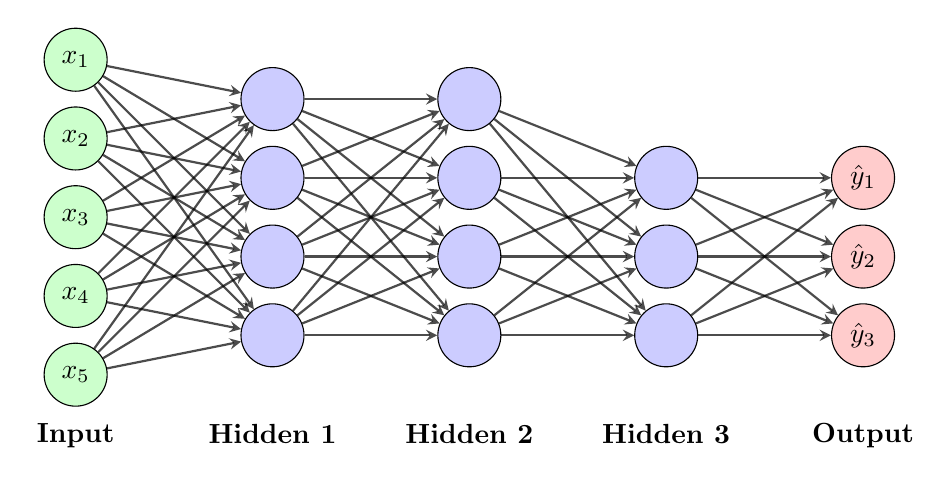
\begin{tikzpicture}[
	node distance=1.5cm and 2cm,
	neuron/.style={circle, draw, minimum size=0.8cm, inner sep=0pt, fill=blue!20},
	input/.style={circle, draw, minimum size=0.8cm, inner sep=0pt, fill=green!20},
	output/.style={circle, draw, minimum size=0.8cm, inner sep=0pt, fill=red!20},
	connection/.style={->, >=stealth, thick, opacity=0.7}
	]
	
	% Input layer (5 nodes)
	\foreach \y in {1,2,3,4,5}
		\node[input] (i\y) at (0, 5-\y) {$x_\y$};
	
	% Hidden layer 1 (4 nodes)
	\foreach \y in {1,2,3,4}
		\node[neuron] (h1\y) at (2.5, 4.5-\y) {};
	
	% Hidden layer 2 (4 nodes) 
	\foreach \y in {1,2,3,4}
		\node[neuron] (h2\y) at (5, 4.5-\y) {};
	
	% Hidden layer 3 (3 nodes)
	\foreach \y in {1,2,3}
		\node[neuron] (h3\y) at (7.5, 3.5-\y) {};
	
	% Output layer (3 nodes)
	\foreach \y in {1,2,3}
		\node[output] (o\y) at (10, 3.5-\y) {$\hat{y}_\y$};
	
	% Connections: Input to Hidden1
	\foreach \i in {1,2,3,4,5} {
		\foreach \j in {1,2,3,4} {
			\draw[connection] (i\i) -- (h1\j);
		}
	}
	
	% Connections: Hidden1 to Hidden2
	\foreach \i in {1,2,3,4} {
		\foreach \j in {1,2,3,4} {
			\draw[connection] (h1\i) -- (h2\j);
		}
	}
	
	% Connections: Hidden2 to Hidden3
	\foreach \i in {1,2,3,4} {
		\foreach \j in {1,2,3} {
			\draw[connection] (h2\i) -- (h3\j);
		}
	}
	
	% Connections: Hidden3 to Output
	\foreach \i in {1,2,3} {
		\foreach \j in {1,2,3} {
			\draw[connection] (h3\i) -- (o\j);
		}
	}
	
	% Layer labels
	\node[below] at (0, -0.5) {\textbf{Input}};
	\node[below] at (2.5, -0.5) {\textbf{Hidden 1}};
	\node[below] at (5, -0.5) {\textbf{Hidden 2}};
	\node[below] at (7.5, -0.5) {\textbf{Hidden 3}};
	\node[below] at (10, -0.5) {\textbf{Output}};
	
\end{tikzpicture}
\end{center}

\textbf{Challenge:} How do we measure if this complex model's predictions are good? \\ 
$\rightarrow$ Same metrics: Accuracy, Precision, Recall, F1-score, Confusion Matrix!

\end{frame}

\section{Regression Metrics}

\begin{frame}{Metrics for Regression: MSE \& MAE}
$$
\bordermatrix{&\text{Prediction}\;(\hat{y})\cr
               &10\cr
               &20\cr
                &30\cr
                &40\cr
               &50}
\qquad \qquad
\bordermatrix{&\text{Ground Truth}\;(\vy)\cr
               &20\cr
               &30\cr
                &40\cr
                &50\cr
               &60}
$$

\begin{align*}
\text{\textcolor{red}{Mean} \textcolor{teal}{Squared} \textcolor{violet}{Error} (MSE)} &=  \frac{\mathcolor{red}{\sum_{i=1}^{n}}(\mathcolor{violet}{\hat{y}_i-y_i)}^{\mathcolor{teal}2}}{\mathcolor{red}{n}} \\ 
\text{Root Mean Square Error (RMSE)} &=  \sqrt{\text{MSE}}
\end{align*}

\end{frame}

\begin{frame}{Accuracy Metrics: MAE \& ME}
$$
\bordermatrix{&\text{Prediction}\;(\hat{y})\cr
               &10\cr
               &20\cr
                &30\cr
                &40\cr
               &50}
\qquad \qquad
\bordermatrix{&\text{Ground Truth}\cr
               &20\cr
               &30\cr
                &40\cr
                &50\cr
               &60}
$$

\begin{align*}
\text{\textcolor{red}{Mean} \textcolor{teal}{Absolute} \textcolor{violet}{Error} (MAE)} &=  \frac{\mathcolor{red}{\sum_{i=1}^{n}}\mathcolor{teal}|\mathcolor{violet}{\hat{y}_i-y_i\mathcolor{teal}|}}{\mathcolor{red}{n}} \\ 
\text{Mean Error} &=  \frac{\sum_{i=1}^{n}(\hat{y}_i-y_i)}{n}
\end{align*}
\pause Is there any downside with using mean error?\\
\pause Errors can get cancelled out

\end{frame}

\popquiz{
\textbf{Why might Mean Absolute Error (MAE) be preferred over Mean Squared Error (MSE)?}
\begin{enumerate}[A)]
	\item MAE is always smaller
	\item MAE is less sensitive to outliers
	\item MAE is easier to compute
	\item MAE works only for classification
\end{enumerate}
}{
\textbf{{\color{magenta}B) MAE is less sensitive to outliers}} since it doesn't square the errors!
}

\section{Summary and Key Takeaways}

\popquiz{
\textbf{For imbalanced datasets, which metrics should you prioritize over accuracy?}
\begin{enumerate}[A)]
    \item Only precision
    \item Only recall
    \item Precision, recall, and F1-score
    \item Only confusion matrix
\end{enumerate}
}{
\textbf{{\color{magenta}C) Precision, recall, and F1-score}} give a more complete picture!
}

\begin{frame}{Key Takeaways}
% \footnotesize
\begin{keypointsbox}{Takeaways}
\begin{itemize}
	\item \textbf{ML vs Traditional Programming:} ML learns rules from data, traditional programming uses predefined rules
	\item \textbf{Features matter:} Choose meaningful features, avoid arbitrary identifiers
	\item \textbf{Classification vs Regression:} Discrete outputs vs continuous outputs
	\item \textbf{Accuracy isn't everything:} For imbalanced data, use precision, recall, F1-score
	% \item \textbf{Visualization is crucial:} Always plot your data (Anscombe's Quartet lesson)
	% \item \textbf{Use baselines:} Simple baseline models help validate your approach
\end{itemize}
\end{keypointsbox}
\end{frame}

\begin{frame}{Summary: Evaluation Metrics}

\scriptsize
\begin{center}
\renewcommand{\arraystretch}{1.3}
\begin{tabular}{|p{2cm}|p{3.5cm}|p{4cm}|}
\hline
\textbf{Task} & \textbf{Common Metrics} & \textbf{When to Use} \\
\hline
Classification & Accuracy, Precision, Recall, F1, Confusion Matrix & 
- Balanced vs. imbalanced data \newline
- Multi-class settings \\
\hline
Regression & MSE, RMSE, MAE, Mean Error & 
- Continuous output \newline
- Check for bias and variance \\
\hline
\end{tabular}
\end{center}

\vspace{0.6cm}
\textbf{Reminder:} \textit{Pick metrics that align with your problem and what matters in practice.}
\end{frame}

\end{document}
